\chapter{Psychoacoustic Characterisation of Rendering Pipelines for Augmented Acoustics}\label{ch:evaluation}
Chapter~\ref{ch:ar-pipeline} demonstrates the engineering process for the implementation of the envisioned proposed pipeline, prototyped on a consumer \acrshort{ar} \acrshort{hmd}. This enables the generation of context-aware auditory stimuli that interact with the physical and virtual scene around the user. The deployment of the pipeline comes at non-trivial computational costs associated with requirements to process scene understanding techniques discussed in Chapter~\ref{ch:materials} for the retrieval of scene acoustic characteristics. Rendering techniques add further requirements to generate acoustic phenomena relative to a given source-listener sound transmission. The costs of the deployment raise the important question: does the computational load justify an increased objective or subjective measure attributed to auditory interactions? \par


\section{Introduction}
Chapter~\ref{ch:acoustic-rendering} discusses increased objective measures evaluated on simulated soundfields and propagated audio. However, it is only by probing human perception that one can address the question concerning subjective measures and justify the computational costs of the engineering process associated with the prototype. With the human listener being the central link of the chain of the proposed system, factors of auditory perception can be investigated to study how acoustic rendering pipelines influence the psychoacoustic response. Perceptive aspects of sound transmissions in immersive applications can affect interactions and activities conducted by the user, especially if such interactions have relationships with spatial characteristics of the environment. The following Sections will investigate psychoacoustic factors of sound transmissions in virtual environments. The proposed acoustic rendering pipeline is tested on an AR device and evaluated by investigating its impact on tasks requiring the application of psychoacoustic abilities. This Chapter tests how well subjects are able to match spatial information provided by an individualised auditory display with holograms projected onto their surroundings. The findings of this chapter describe how an acoustic spatialisation workflow applied to a common teaching room has a significant impact on ability in common psychoacoustic tasks as opposed to a no acoustic spatialisation condition.

% contributions
This Chapter contributes towards:
\begin{enumerate}
    \item the presentation of a novel methodology for studying psychoacoustic factors of sound transmissions between sound sources and a human listener within a simulated soundfield displayed in augmented reality;
    \item the development of a novel bespoke testing framework for conducting a user evaluation in augmented reality using a custom audio engine and a prototype acoustic rendering pipeline;
    \item outlining recommendations for future designs of audio rendering pipelines for immersive technology drawing from a dataset of perceptual responses captured from a user study on two tasks dependent on psychoacoustic abilities.
\end{enumerate}

\section{Methodology}
\begin{figure}[htbp]
    \centering
    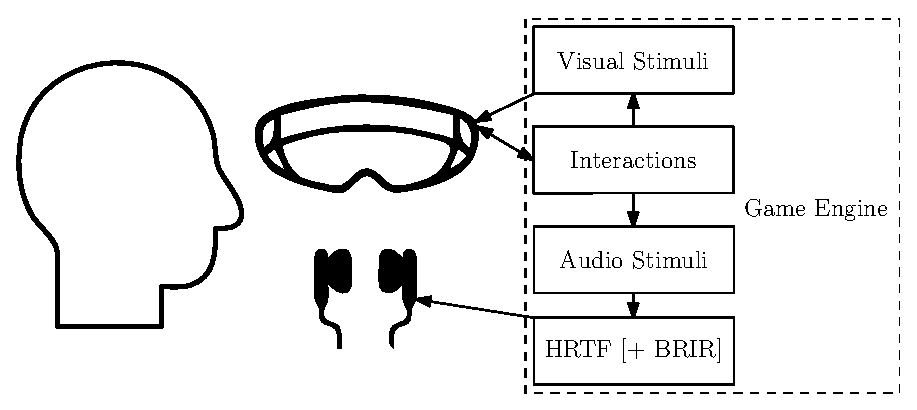
\includegraphics[width=1\linewidth]{pshyco-apparatus}
    \caption[Apparatus overview for psychoacoustic testing]{The experimental apparatus used to implement the testing framework and execute the two tasks, \emph{localisation} and \emph{clustering}, administered to recruited participants.}\label{fig:psycho-apparatus}
\end{figure}

\subsection{Overview}
This evaluation aims at investigating how audio interactions in \acrshort{ar} affected by simulated acoustic phenomena influence task perfomance in complex scenes. The methodology evaluates tasks that are dependent on psychoacoustic abilities, such as pinpointing the location and resolving the direction of arrival of sound sources or determining the number of concurrent sound sources at varying angular distances between sources. To investigate these factors, a within-subjects evaluation is designed to probe the human auditory perception applied to practical tasks in a virtual environment. Localisation of sound-emitting objects is set as the primary psychoacoustic-related task affecting task performance in immersive environments, followed by testing the ability to detect clustered sound sources, as source clustering is a key factor in sound propagation system design for complex scenes that are typical of AR applications \citep{schissler2016interactive}. 


\subsection{Task Definitions}
\begin{figure}[htbp]%procedure diagram
    \centering
    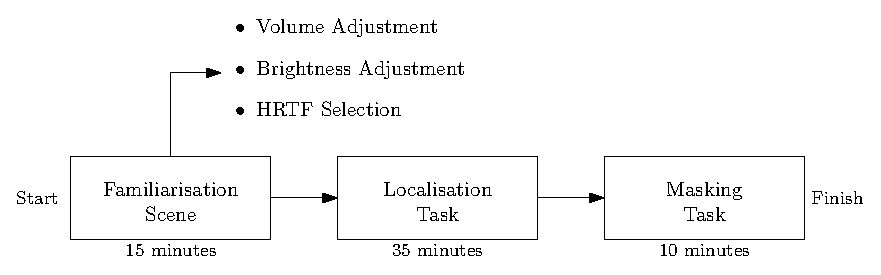
\includegraphics[width=1\linewidth]{procedure-overview}
    \caption[Overview of psychoacoustic experiment procedures]{Experiment procedure administered to participants: the task starts with a familiarisation scene where the user is introduced to the UI system and is asked to calibrate the audio reproduction system. The user then performs the localisation and masking tasks after the familiarisation scene.}\label{fig:psycho-procedure-overview}
\end{figure}
The subjective study is administered to participants as an \acrshort{ar} application, see Figure~\ref{fig:psycho-procedure-overview} and focuses on two tasks that are:
\begin{enumerate}
    \item the \textbf{localisation} task: where participants are asked to listen to a set of audio stimuli and indicate which holographic object is responsible for emitting each stimulus, choosing from arrays of holographic objects;
    \item the \textbf{masking} task: where participants are displayed concurrent audio stimuli, and they are asked to determine whether these propagate from a singular or two invisible sound-emitting objects.
\end{enumerate}
The rationale for defining the tasks centre around key aspects of sound rendering, namely the efficacy of propagation effects, measured by analysing user performance in tasks requiring the perception of spatial clues encoded in audio transmissions presented to the users within the complex scene. The other aspect centres around the problem of performance the limited computational resources in \acrshortpl{hmd}.
The localisation task aims at evaluating whether there is a significant increase in perceived spatial information using a sound rendering pipeline, compared to unpropagated stimuli. This task is often evaluated to analyse the effectiveness of sound rendering methods \citep{rungta2016psychoacoustic}.
The masking task measures how concurrent sound sources are perceived by the user, studying the efficacy of sound rendering pipelines in resolving masking effects occurring in sound sources at varying distances from each other. Testing how users perceive concurrent sound sources can provide insights and guidelines for handling clustered sources in large-scale scenes, aiming at reducing the load of propagation methods simulating multiple sources \citep{schissler2016interactive}.
Section~\ref{sec:psy-procedure} details the procedure repeated for each participant to conduct the two tasks.

\subsection{Participants}
31 participants, of whom 16 females and 15 males, were recruited from staff and students of Birmingham City University and were invited to partake in the two tasks, which are defined as follows. Participants were asked to pinpoint the location of a set of sounds, resolving the direction of arrival of sound sources and determining the number of concurrent sound sources they could identify at varying angular distances. A within-subjects design was conducted with 31 participants (16 females, 15 males) to probe the human auditory perception of practical tasks in a virtual environment.

\subsection{Apparatus and Evaluation Platform}
\begin{figure}[htbp]%room mesh
    \centering
    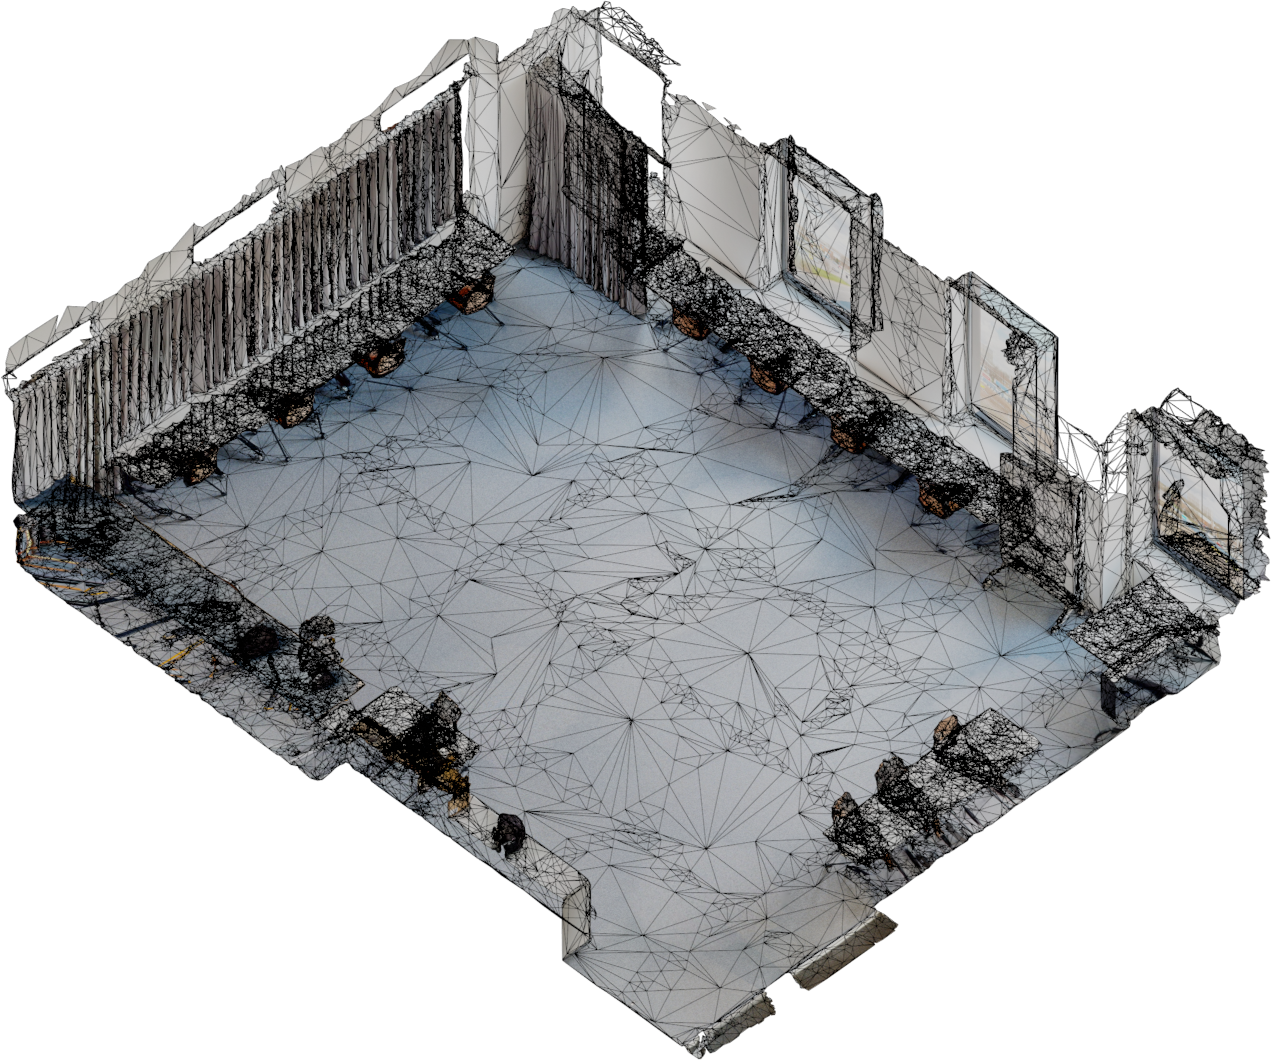
\includegraphics[width=1\columnwidth]{cst_isoview}
    \caption[Virtual reconstruction of the physical space used for psychoacoustic testing]{Visualisation of the virtual reconstruction of the space used for the user study. The space, scanned using a Matterport Pro3 camera, is manually segmented into semantically related portions of geometry aligning with acoustic material definitions (e.g.\ curtains, floor, walls) and imported into the game engine for scene alignment and spatial mapping. The scanned geometry is handled using a Bounding Volume Hierarchy to allow indexing and searching of the triangle primitive for acoustic material tagging and rendering operations. Acoustic rendering is performed between sources and the listener, generating impulse response pairs, based on propagation paths computed by a ray tracer bouncing rays off the scene geometry with tagged acoustic materials.}\label{fig:cst-mesh}
\end{figure}
The two tasks were implemented in Unity 2021.3.14f1 and deployed and executed in a Microsoft Hololens 2 HMD\textsuperscript{\ref{note:ms-hl2},\ref{note:ms-hl2-hw}}. Figure~\ref{fig:psycho-apparatus} shows the experimental apparatus composing the evaluation framework: the user is presented with visual and auditory stimuli driven by the Unity game engine, responsible for managing the scene representing the evaluation tasks, rendering holographic interactable objects. Audio reproduction was done through the embedded audio interface in the Microsoft Hololens 2 HMD and using a pair of Bose Soundsport earbuds with an integrated D/A converter.\par
Spatial information relating to the scene and the user, as well as interactions detected by the gesture recognition features of the HMD, determine the reproduction of audio stimuli. These are processed with customised spatialisation tools to consider human factors in the audio reproduction chain. The system is tested in a real space, a teaching room of $10.7m$ by $8.6m$ dimensions, where participants stand in the middle of the room wearing the HMD and a headset to complete the two tasks with their freedom being restricted to 3 DoF.\par

\subsection{User Interface System}
The testing apparatus incorporates a diegetic user interface integrated within the immersive environment. Diegetic UI elements exist within the narrative world of the AR experience, creating a sense of immersion for the user. This approach has been proven to increase user engagement and realism by making the UI elements a part of the user's surroundings, rather than overlaying non-diegetic elements that can disrupt the task \citep{dickinson2021diegetic}.
The UI for the subjective testing was designed using the Microsoft Mixed Reality Toolkit (MRTK)\footnote{\url{https://learn.microsoft.com/en-us/windows/mixed-reality/develop/unity/unity-development-overview}}. MRTK provides a comprehensive collection of components and features that simplify the development of AR applications. Leveraging MRTK allowed for the creation of intuitive and responsive UI elements, ensuring a consistent and high-quality user experience. The toolkit's support for spatial interactions and holographic elements was crucial in developing an interface that could dynamically adapt to the user's movements and interactions within the AR environment. The toolkit is used to create panels and controls for participants to adjust audio settings, such as volume or current \acrshort{hrtf}, see Figure~\ref{fig:test-participant-perspective}.\par
Sound sources in the localisation task (later illustrated by Section~\ref{sec:localisation-task-procedure}) are visually displayed to the user through virtual cubes arranged in three circular arrays corresponding to different distances: near, medium, and far. Each array represented a specific proxemic zone, which is crucial for understanding how users perceive and interact with sound sources in AR. 
Proxemics zones relate to physical distance as a dimension of interaction design, where the spatial relationship between users and devices influences interaction possibilities \citep{huang2022proxemics}. In the near array, the inner circle of holographic cubes was placed within the personal space of the user, which is defined to be approximately \qty{0.5}{\metre} to \qty{1.5}{\metre}. This distance represents close interactions where sounds are expected to be more intimate and directly related to the user. The medium distance array has cubes positioned within the social space, around \qty{1.5}{\metre} to \qty{4}{\metre} meters from the user. This zone corresponds to social interactions where sounds need to be clearly audible but not as intimate as those in the personal space. The outer circle is placed within the public space, at \qty{4}{\metre} distance or farther. Sounds originating from this distance are meant to represent broader environmental audio, providing context without being the primary focus \citep{buschel2021miria}.

\subsection{Geometry Reconstruction and Handling}
The room, the physical test environment, is scanned using a Matterport Pro3\footnote{\url{https://matterport.com/pro3}} camera, from 9 camera placements covering the walkable space of the room uniformly, with the Near array being $0.9m$ from the listener, the Medium $2.24m$, and the Far $4.02m$;  refer to Figure~\ref{fig:cst-mesh} for a visualisation of the mesh showing wireframe geometry and textures of the reconstruction. The textured triangulated mesh is partitioned into semantically related segments, separating architectural components of the room, as well as furniture and objects, into individual meshes to facilitate indexing and attributing of physical characteristics to portions of the scene geometry. Portions of the segmented are tagged attributing frequency-dependent absorption coefficients and mapping the appearance of the reconstructed textures with acoustic materials from measured absorption data\footnote{\url{https://odeon.dk/downloads/materials/}}, see Figure~\ref{fig:cst-208-materials}. In acoustic rendering operations, material properties assigned to scene geometry are required to approximate models of the environment soundscape. 
In the testing framework, the reconstructed geometry is used by the game engine to align holographic objects with the physical space. We use a dynamic \acrshort{bvh} implementation, constructing the tree using mesh triangles with attributed acoustic absorption characteristics to organise, index, and search the scanned geometry within the game engine for sound propagation \citep{kopta2012fast}.\par

\subsection{Acoustic Rendering Apparatus}
\begin{figure}[htbp]
    \centering
    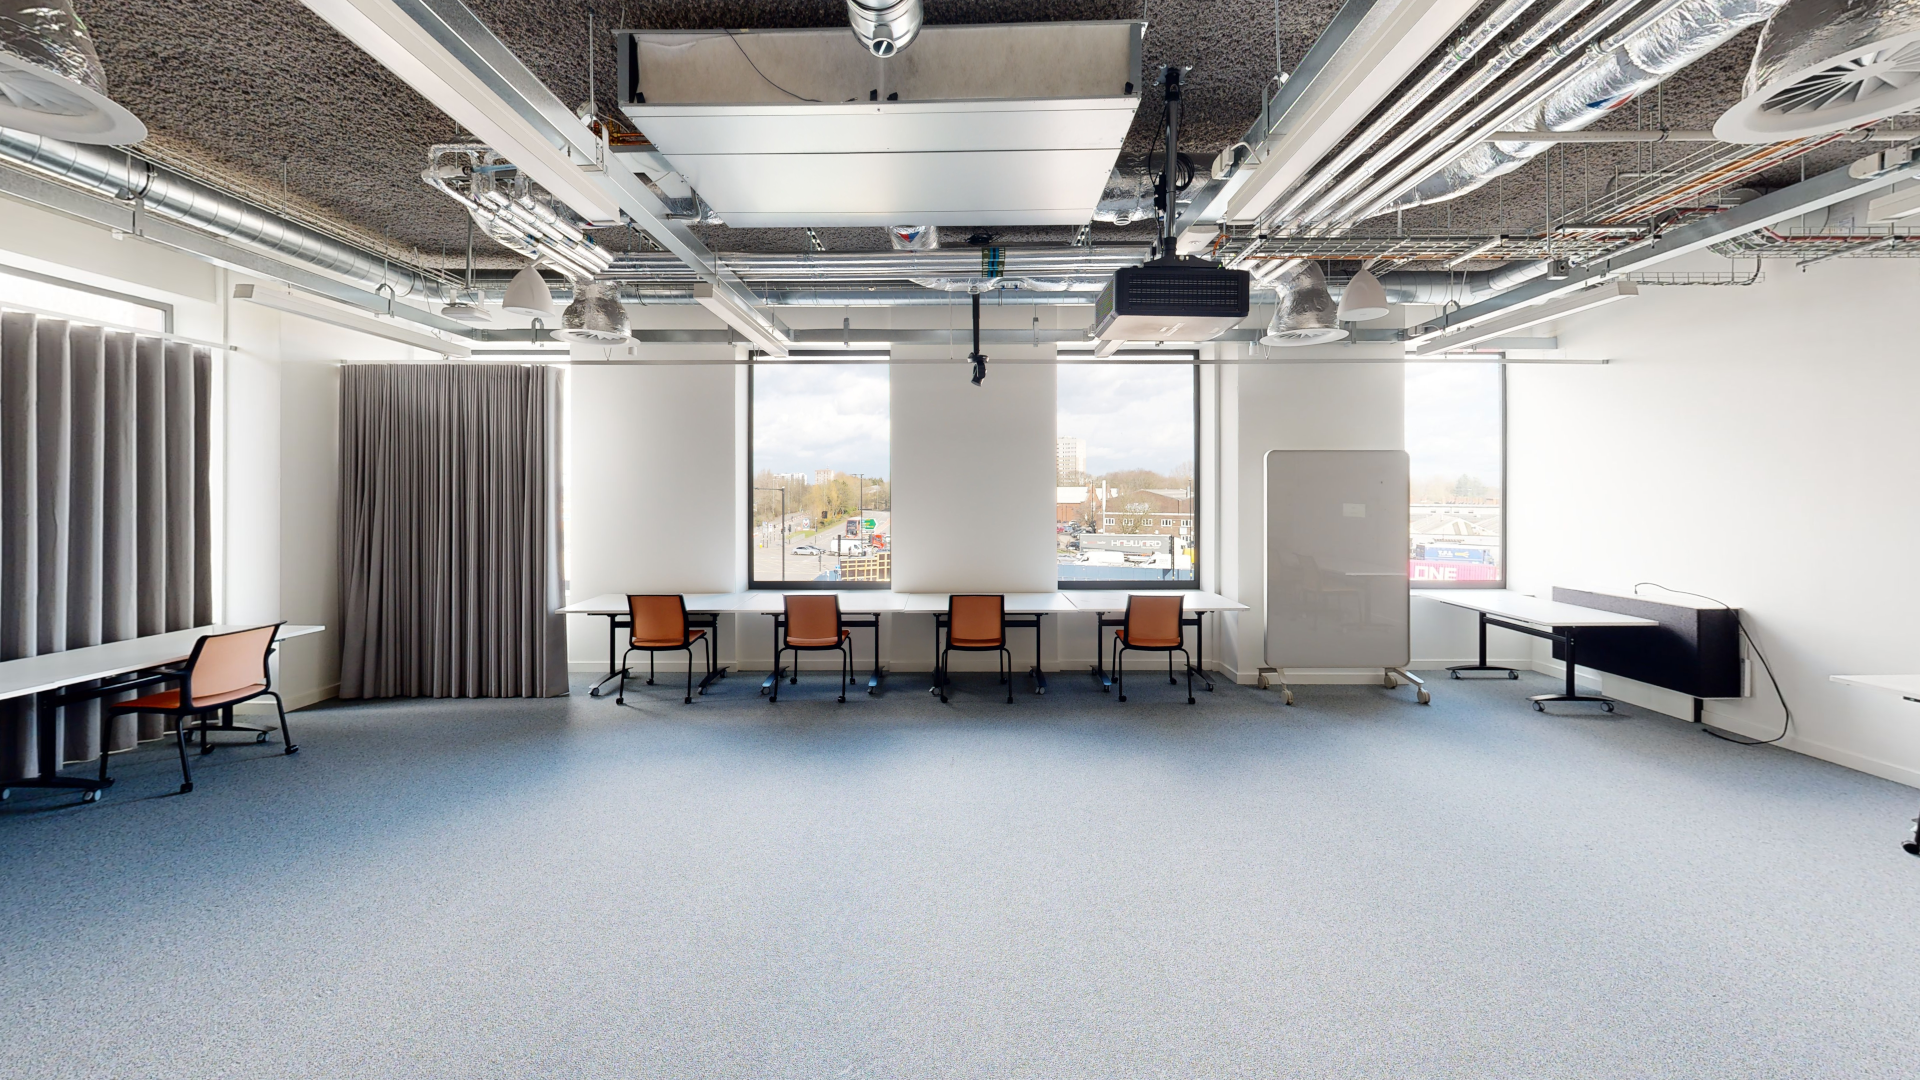
\includegraphics[width=1\linewidth]{CST-208-2}
    \caption[Physical space used for psychoacoustic testing]{A photograph of a teaching space used for deploying and testing an implementation of the proposed system.}\label{fig:cst-208-photograph}
\end{figure}
The experimental evaluation deploys the rendering pipelines presented in Chapter~\ref{ch:ar-pipeline} as an offline process. The soundscape is simulated by generating \acrshort{ir} for source-listener pairs in the AR environment by implementing the renderer proposed in Section~\ref{sec:ga-based-pipeline}, maintaining the validity of the offline renders by adopting static sound sources and environment and limiting the movement freedom of the listener. As shown in Figure~\ref{fig:psycho-apparatus}, auditory stimuli use \acrshortpl{rir} convolved to anechoic audio samples to reflect approximated acoustic phenomena in audio signals displayed to participants. The experimental evaluation uses ray tracing as an offline rendering to perform sound propagation between scene elements in \acrshort{ar}. This is done by restricting sound transmissions to static sound sources and a static listener (the participant). Hence, the participant's position is fixed within the grey holographic barriers, as shown in Figure~\ref{fig:psycho-top-view}.
We implement a minimal geometrical acoustics renderer, based on \cite{saviojaGA}'s work, to approximate reverberation by modelling acoustic energy decay with propagation paths between an emitter and detector. Sound sources are considered omnidirectional emitters, from which $3*10^3$ rays originate at uniformly distributed points on a $1m$ radius sphere located at the sound source position in the scene, searching for geometrical intersections within the \acrshort{bvh} constructed on the scanned space, see Figure~\ref{fig:cst-mesh}. Intersections are computed between propagating rays and leaf nodes of the \acrshort{bvh}, using the normal and acoustic absorption data attributed to the encapsulated triangle, allowing propagation paths a maximum of four reflection orders.
$\alpha_f$ acoustic absorption data provided by tagged materials and attributed to mesh triangles is frequency-dependent, $f \in \{ 125, 250, 500, 1000, 2000, 4000 \}Hz$, following state-of-the-art sound propagation methods \citep{schissler2017acoustic}.\par
\begin{figure}[htbp]
    \centering
    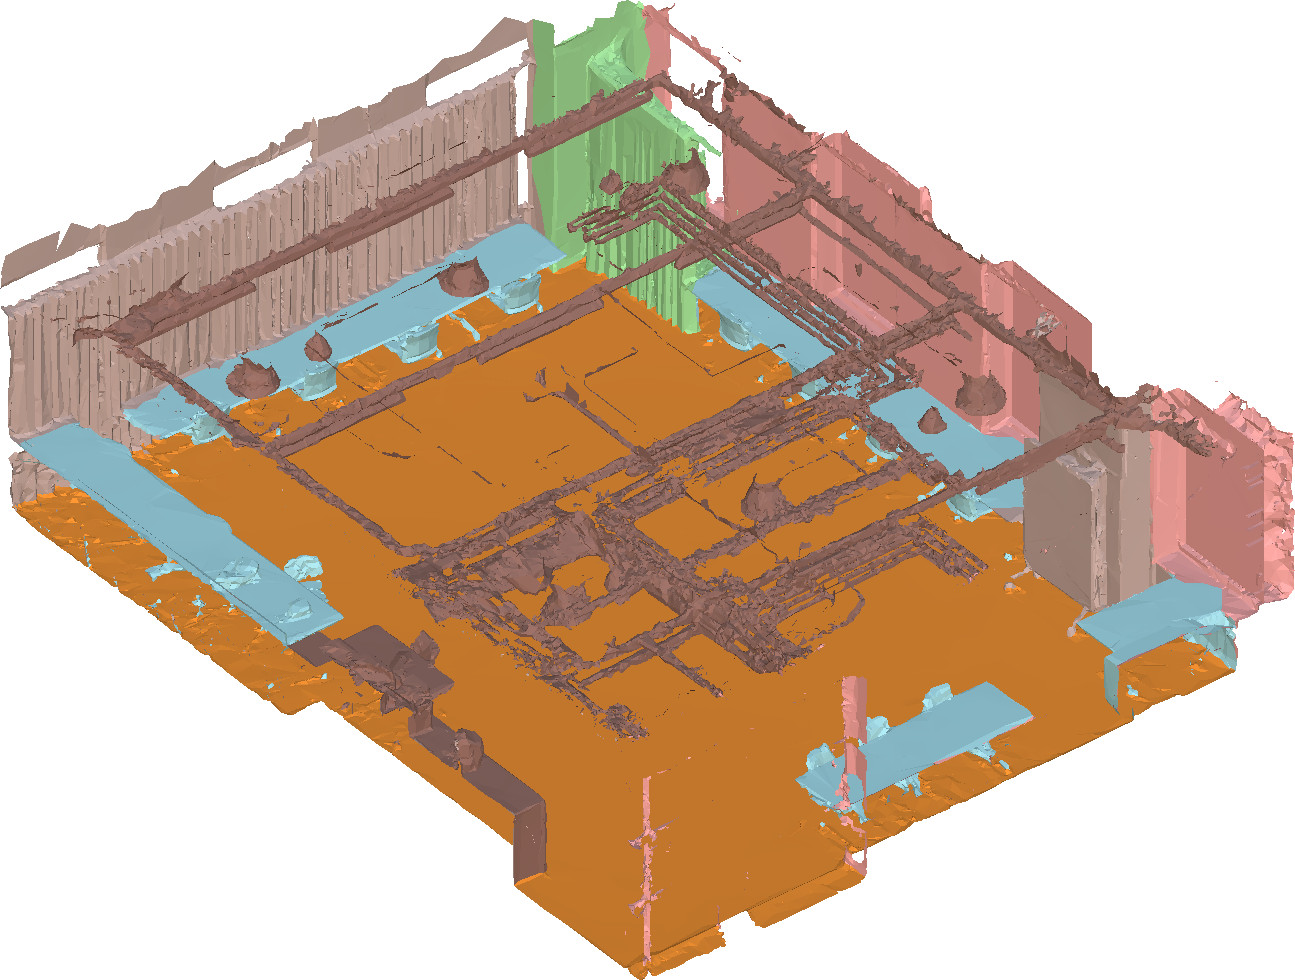
\includegraphics[width=1\linewidth]{CST-208-mats} \\
    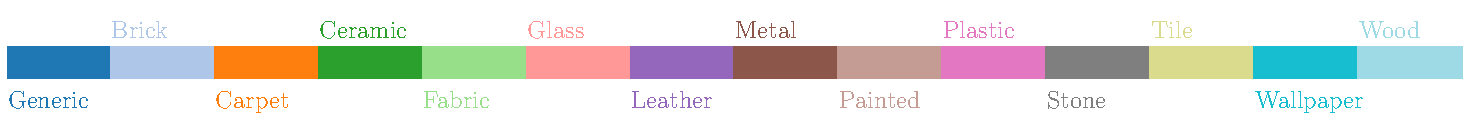
\includegraphics[width=1\linewidth]{cst-mat-vis}
    \caption[Acoustic material visualisation of space for psychoacoustic testing]{An isometric view of the room used for the experiment, visualising acoustic materials. Materials are mapped to the scanned environment geometry (see Figure~\ref{fig:cst-mesh}) by segmenting the mesh into semantically meaningful submeshes that represent scene entities.}\label{fig:cst-208-materials}
\end{figure}
Propagation paths have $e_0 = 1$ initial energy values across six frequency bands relating to frequency-dependent material data, attenuated upon collisions with scene geometry and logged in a series of \acrshortpl{ir} that model frequency-dependent reverberation. To overcome the deterministic nature of the ray tracer, we adopt \cite{schroder2011physically}'s technique, consisting of generating Poisson-distributed sequences of Dirac-Delta pulses to simulate the likelihood of detecting acoustic reflections in a hypothetical environment. These sequences are convolved with the modelled energy from the ray tracer, filtered based on their respective frequency band contributing towards Equivalent Rectangular Bandwidths (ERB) portions of the spectrum centred around each $f$ and having all frequency-dependent \acrshortpl{ir} contributing equally towards the spectrum, which are finally summed together into a \acrshort{rir}.\par
Listener and sound source positions were pre-determined by the \emph{localisation} and \emph{clustering} task, see Figure~\ref{fig:psycho-top-view}; RIRs are pre-computed for all sound-emitting objects placed in the virtual reconstruction of the space.

\subsection{Audio Rendering Apparatus}\label{sec:audio-apparatus}
The pre-computed RIRs associated with the sound-emitting objects placed in the test scenes were combined with sets of Head-Related Impulse Responses (HRIRs). These were drawn from the public CIPIC database in real-time by implementing a fast convolution engine. This engine convolves RIRs and Head-Related Transfer Functions (HRTFs) with audio signals, creating two types of audio stimulus sets $S$: 
\begin{align}
     \forall y \in S_{A}\ & y_l(t) = x(t) * h(\theta, \phi, t)\\
     & y_r(t) = x(t) * h(\theta, \phi, t) \\
     \forall y \in S_{P}\ & y_l(t) = x(t) * RIR(t) * h(\theta, \phi, t) \\
     & y_r(t) = x(t) * RIR(t) * h(\theta, \phi, t)
\end{align}
where $t$, $\theta$ and $\phi$ indicate, respectively, time, the listener's azimuthal position and elevation. HRTFs are interpolated in real-time using AES SOFA containers \cite{hoene2017mysofa} and computed based on the listener's head orientation determined by the HMD tracking system. The final links of the audio reproduction chain consist of the embedded audio interface in the Microsoft Hololens 2 HMD that provides a display to the user via a pair of Bose Soundsport earbuds with an integrated D/A converter.\par
\begin{figure}[htbp]
    \centering
    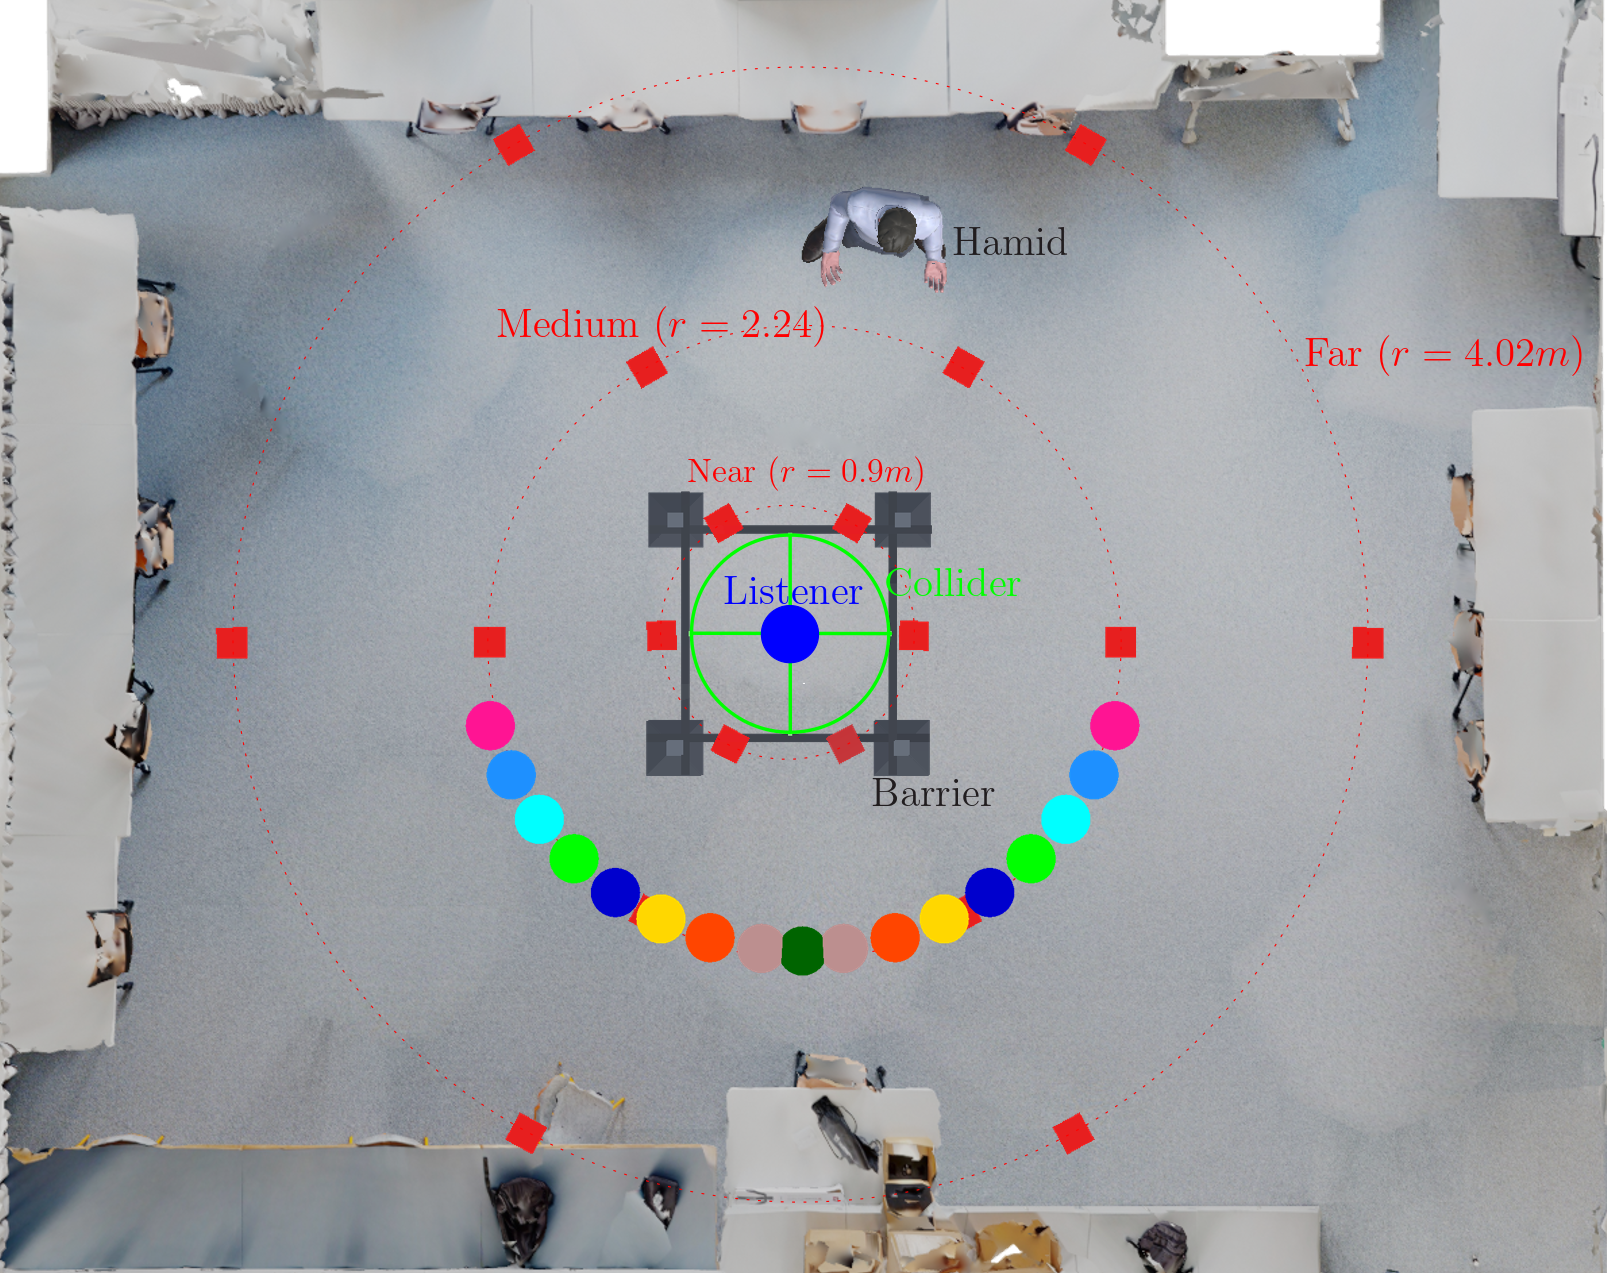
\includegraphics[width=1\linewidth]{cst208topview-diagram2}
    \caption[Psychoacoustic testing diagram --- top view]{Top view of the testing environment overlaid on a top view photograph of the room used for running the user study. The overlay shows the listener at the centre of the room, the blue dot, surrounded by an invisible collider, visualised as a green wireframe, to detect and warn the participant moving outside the bounds. Crowd barriers, the grey objects surrounding the listener, restrict the participant's movement. The red objects visualise the holographic sound sources for the sound localisation task procedure. The circular \emph{Near}, \emph{medium}, and \emph{far} arrays are visualised with dotted circles, indicating the distances from the user, respectively, $0.9$, $2.24$, and $4.02m$. All holographic cubes have a $60^\circ$ angle of distance between each other.}\label{fig:psycho-top-view}
\end{figure}

\subsection{Audio Stimuli}
\begin{figure}[htbp]
    \centering
    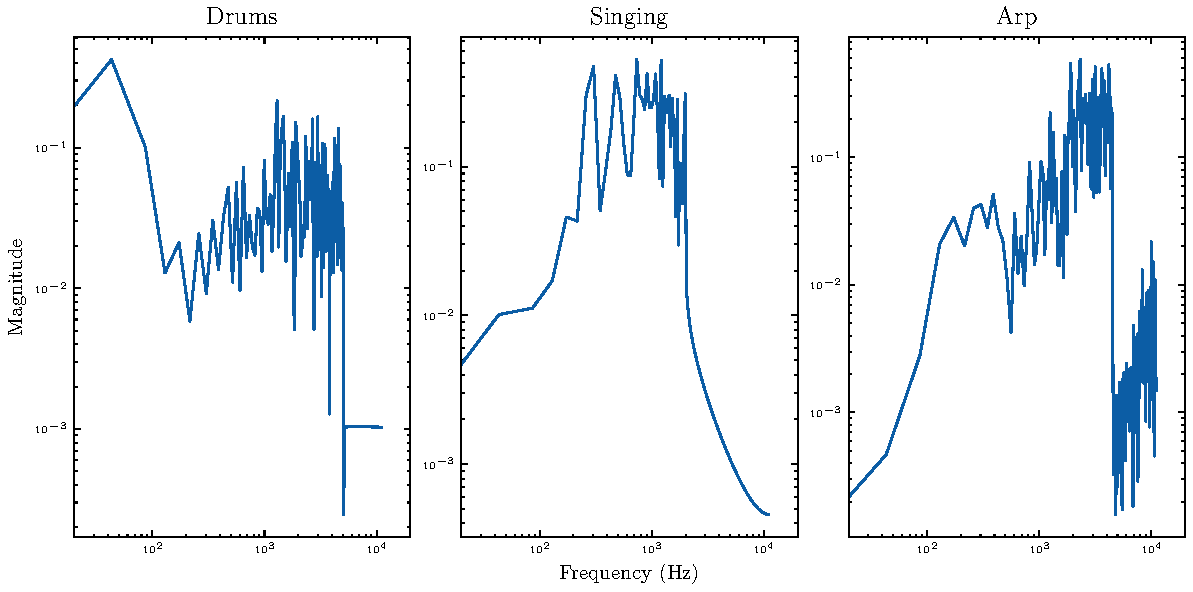
\includegraphics[width=1\columnwidth]{stimuli}
    \caption[Visualisation of audio stimuli used in psychoacoustic tests]{The evaluation design uses three auditory stimuli, reproduced as spatialised sound sources placed at positions defined by the near, medium, and far array. The figure shows a spectral analysis conducted over the three stimuli showing how the spectrum of ``drums'', ``singing'', and ``arp'' centre around low, medium, and high frequencies.}\label{fig:stimuli}
\end{figure}
The testing framework presents two sets of audio stimuli: a \emph{set} of anechoic audio excerpts $S_A$, and a \emph{set} containing corresponding audio excerpts $S_P$ generated using a prototype deployment of the geometrical acoustics pipeline. The latter set of auralisations is produced based on the listener's position during the testing procedure and the position of the sound-emitting objects in the testing scene. \par
In localisation test methods, it is common to use test tones or broadband noise as stimuli to evaluate the distance between ground truth source positions and target positions expressed by participants \citep{bertet2013investigation, kashino1998adaptation}. Psychoacoustic factors around the perception of loudness may affect the application of localisation abilities \citep{blauert1997spatial}. Hence, stimuli are selected to cover a wide range of frequencies around the audible range.
For the \emph{localisation} task, both sets are constructed with three anechoic audio samples: a $4.98s$ drums loop, a $4.87s$ singing clip, and a $7.14s$ violin clip. All sound clips are indefinitely looped until the subtask is completed or the participant pauses them with interactable panes presented every time audio is reproduced.
The \emph{clustering} task has eight pairs of $25s$ multi-instrument anechoic recordings\footnote{\url{https://odeon.dk/downloads/odeon-zip-archives/}}. For each pair, the two sound sources emit a different instrument from the same musical excerpt. Emitting the same audio from the two sources is avoided to prevent potential reproduction artefacts of phase cancellations that could interfere with the task. The \emph{clustering} task has eight anechoic pairs, and eight counterparts propagated with appropriate IRs for a total of 18 subtasks.

\subsection{Procedure}\label{sec:psy-procedure}
Each study lasted between 60 and 90 minutes, the study protocol had the approval of the Institutional Review Board. The study was broken down into the following steps. Informed consent, including experience, was attained from participants prior to each study session. After welcoming participants, the purpose of the study and test protocol was explained in detail. The researcher then measured visual acuity and colour blindness via a Snellen chart and Ishihara test. Participants were then asked to adjust and wear the HMD, so it was comfortable and stood at the initial starting position. 

\subsubsection{Familiarisation Scene}
\begin{figure}[htbp]
    \centering
    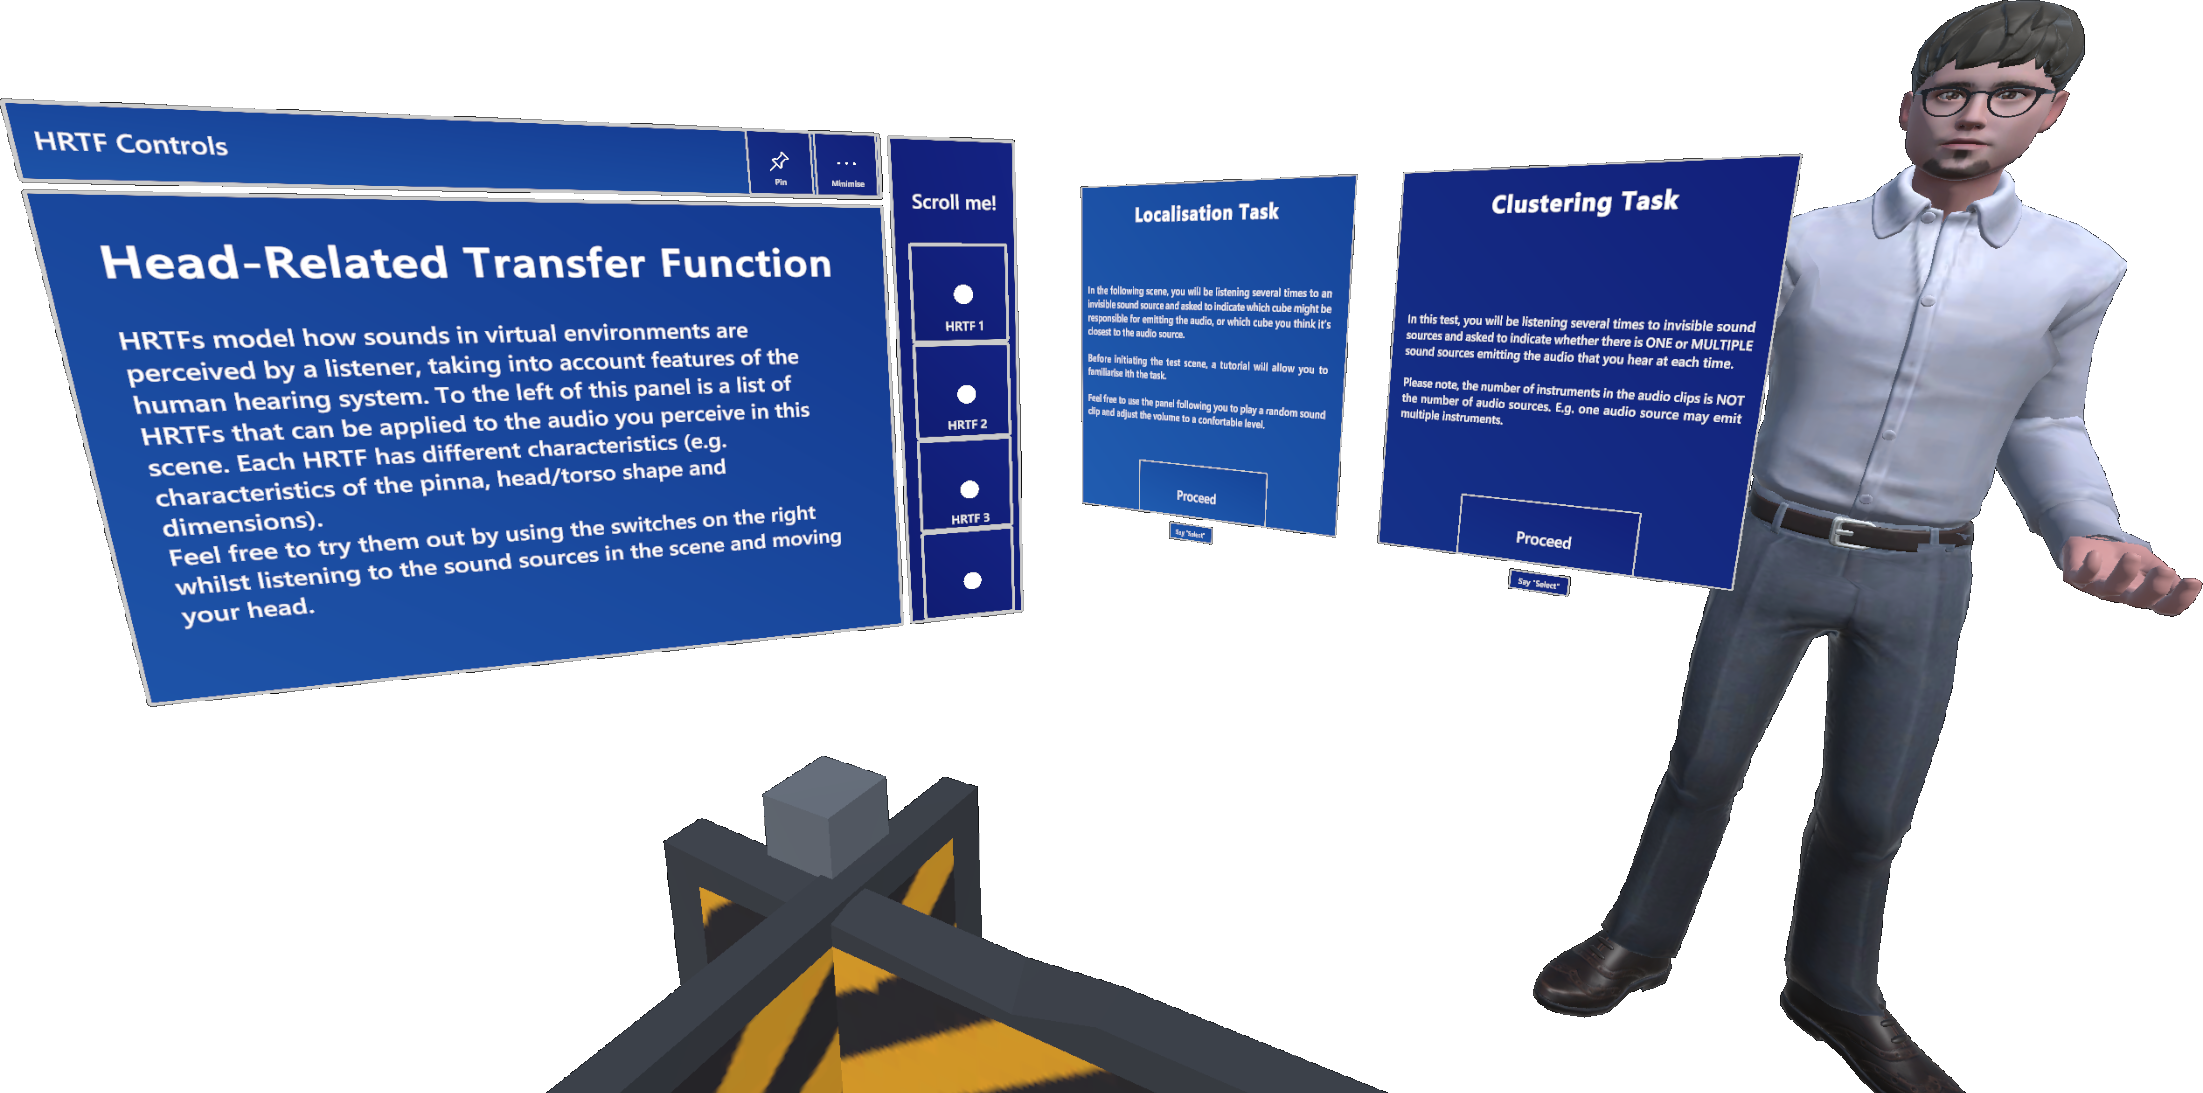
\includegraphics[width=1\linewidth]{test_participant_perspective}
    \caption[Participant's perspective of psychoacoustic testing --- familiarisation]{A frame from the render buffer displayed to the user through the Microsoft Hololens 2 Head-Mounted Display: the frame shows the holographic content displayed to the participant when entering the testing environment, consisting of, from left to right, a set of interactive panels for Head-Related Transfer Function explanations and controls; two sets of panels for learning and accessing the two tasks, localisation and masking; a virtual hologram of Hamid, a spatialised sound-emitting character briefing and summarising key information to the participant. At the bottom is a portion of the crowd barrier object that limits the participant's freedom of movement.}\label{fig:test-participant-perspective}
\end{figure}
The testing framework introduces the participant to the tests via a familiarisation scene composed of panels to describe and allow access to the two tasks, barriers to limit the participant's freedom of movement, a panel to explain and control the spatialisation system, and a sound-emitting hologram. The sound-emitting hologram, visualised in Figure~\ref{fig:psycho-top-view} as the character ``Hamid'', emits a $102s$ long anechoic recording of a narration summarising knowledge on spatialised audio and the nature of the two tasks; the recording is looped indefinitely until the participant pauses it with panel controls or enters any of the tasks. Users are asked to use this scene to adjust and calibrate the audio-visual setup, ensuring they are comfortable with the tasks and the controls of the User Interface. \par
%There are volume and brightness controls available, provided by both the test interface and the HMD, allowing subjects to calibrate the loudness of audio signals and visibility of holograms using the example sound-emitting hologram. 
A panel briefs subjects on the basic features of the audio spatialiser system, allowing the selection of different HRTF containers, see Figure~\ref{fig:test-participant-perspective} for a first-person view render of the panel. There are 10 available HRTF selections drawn from the CIPIC database, as described in Section~\ref{sec:audio-apparatus}. These are sampled uniformly to represent the anthropometric spectrum of the database. There are no time constraints to the familiarisation scene, and subjects are asked to test each HRTF selection with the sound-emitting hologram until they find the selection that allows the best perceptive visual-acoustic spatial matching. After the familiarisation task was complete, participants were then asked to proceed to the study tasks, with half of them completing the localisation task first and the other half starting with the source clustering tasks.\par

\subsubsection{Localisation Task}\label{sec:localisation-task-procedure}
\begin{figure}[htbp]
    \centering
    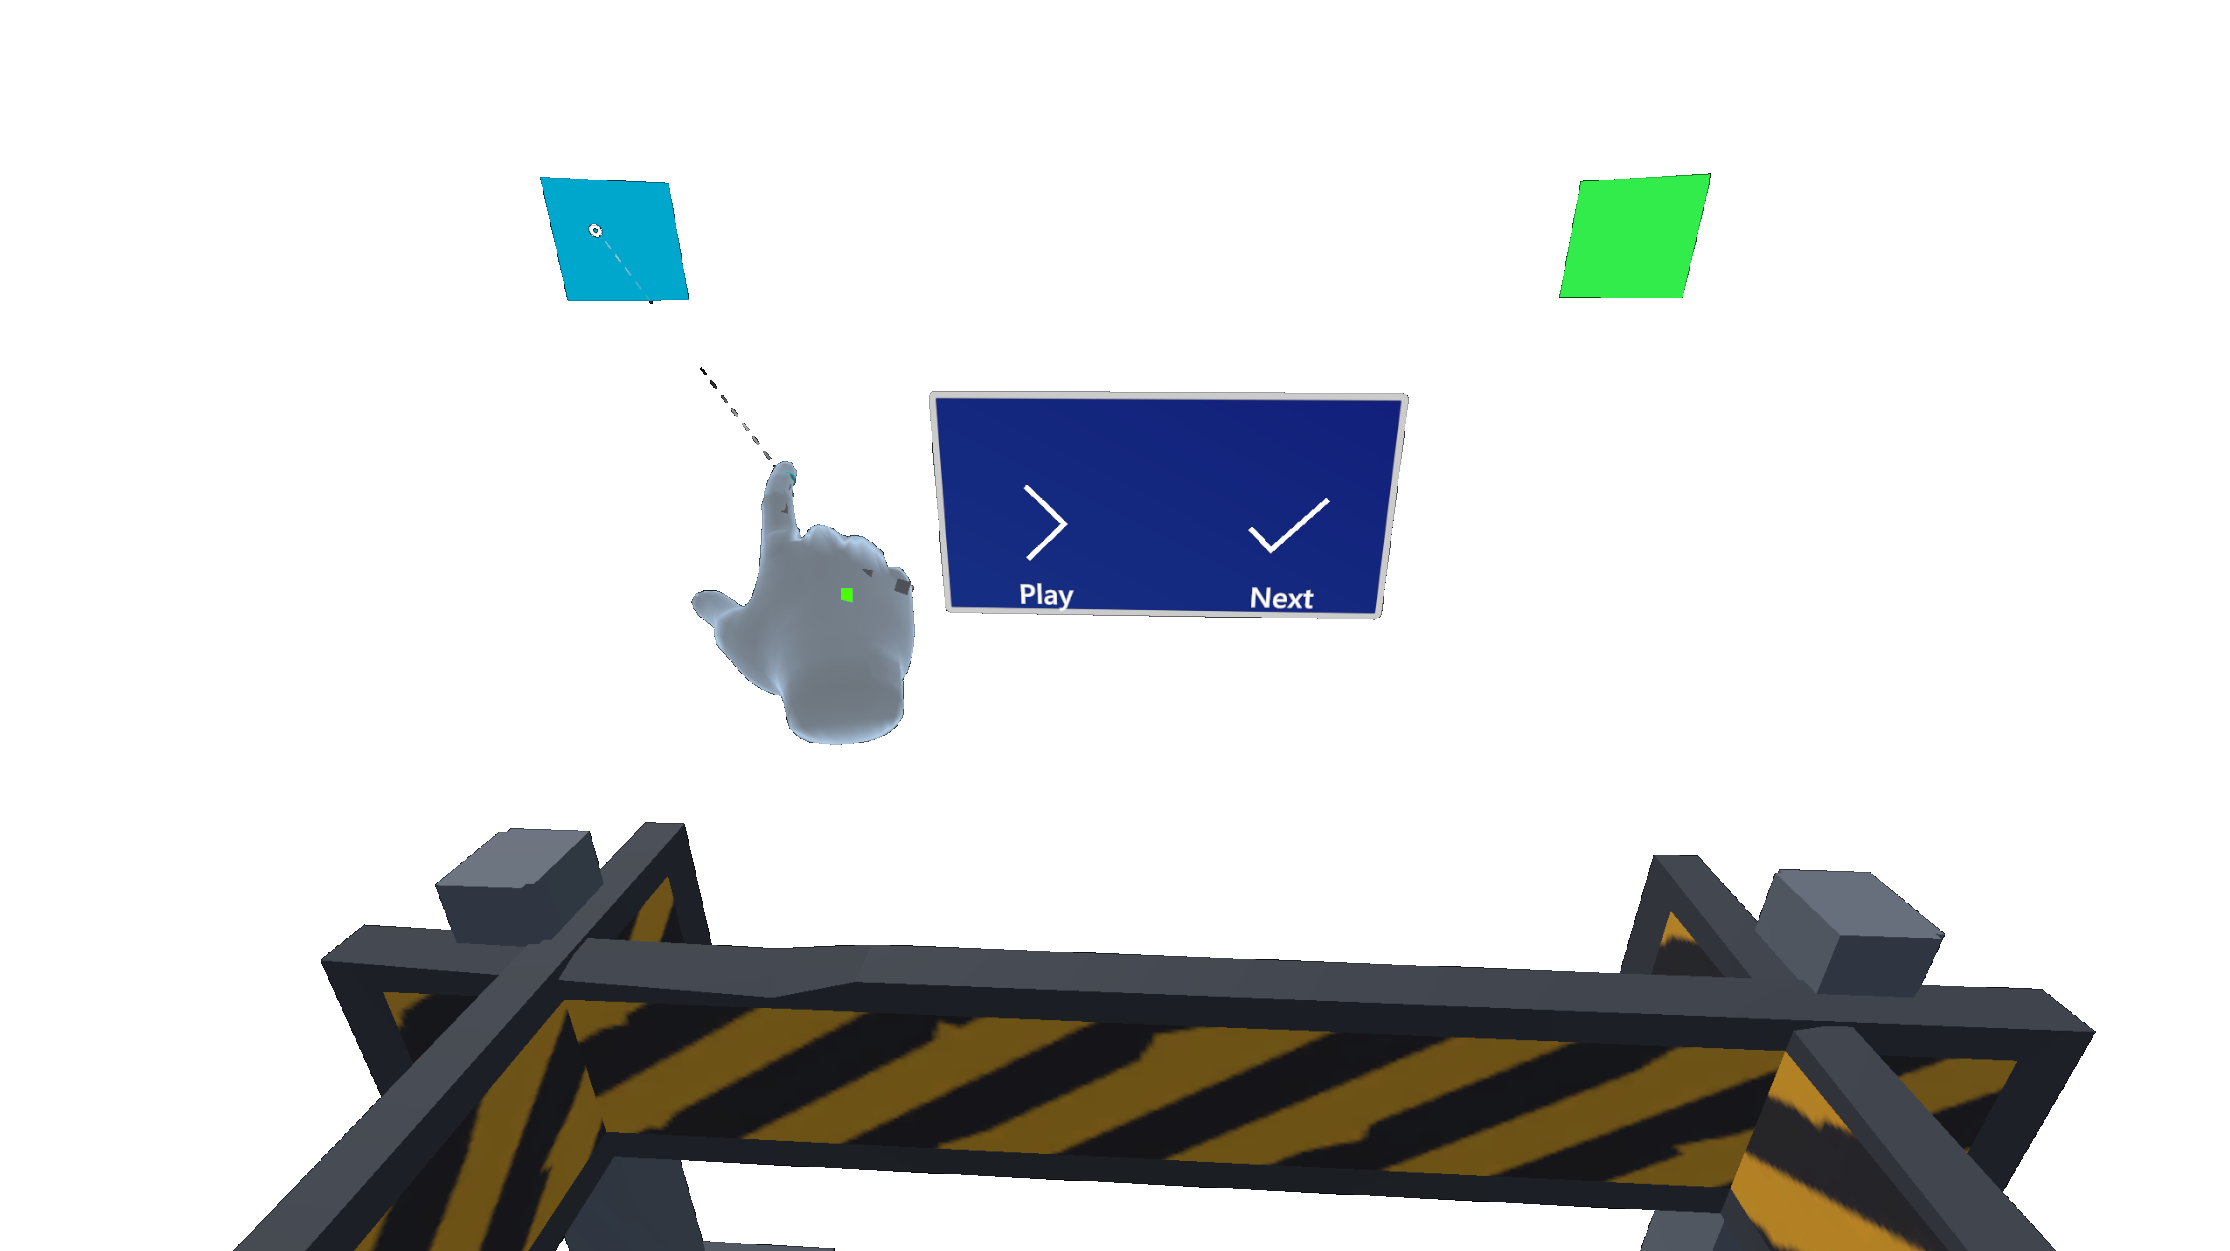
\includegraphics[width=1\columnwidth]{localisation-fpv}
    \caption[Participant's perspective of psychoacoustic testing --- localisation]{First-person view of the localisation task: the participant, surrounded by circular arrays of sound-emitting cuboids, perceives spatialised audio and is asked to determine which of the holographic cubes is responsible for emitting sounds. The participant selects the cube that best matches the spatial position and direction conveyed by the auditory information by indicating with their hands, tracked by the HMD.}\label{fig:localisation-fpv}
\end{figure}
The goal of the \emph{localisation} task is to evaluate the success rate of participants identifying the hologram responsible for emitting audio stimuli that are displayed via a bespoke sound system. \par
The procedure starts with the participant standing on the marker indicated on the floor, within the holographic barriers in the virtual testing environment; a holographic panel presents a quick summary of the tasks and asks whether the participant is ready to proceed. Upon interaction with the proceeding button on the panel, the first circular array of sound sources, the \emph{near} array, is projected via the HMD around the user as static red cubes elevated at $1.4m$, a standard altitude adopted in source-receiver measurements in soundfield. With the array of sound sources around the user, a spatialised audio stimulus is displayed through the sound reproduction setup; the participant is tasked with indicating the holographic cube they deem responsible for emitting the stimulus. The cube tint transitions from red to green, indicating the user's selection. The stimulus is reproduced in a loop, without time limits, until the user proceeds to the successive stimulus using a panel always shown in front of the user. The stimuli are drawn randomly from both sets $S_A~\cup~S_P$.\par
The task has three phases: the near array, the medium array, and the far array. These arrays are distributed across the walkable radius of the testing room, see Figure~\ref{fig:psycho-top-view}. All phases have six sound-emitting objects, each emitting six stimuli, the three anechoic audio clips and three corresponding propagated clips. Hence, each participant is presented with 108 stimuli. For all three phases, participants were to complete all subtasks. For each subtask, an auditory stimulus was presented, drawing from a shuffled set of anechoic and propagated audio clips associated with each phase. \par

\subsubsection{Clustering Task}
\begin{figure}[htbp]
    \centering
    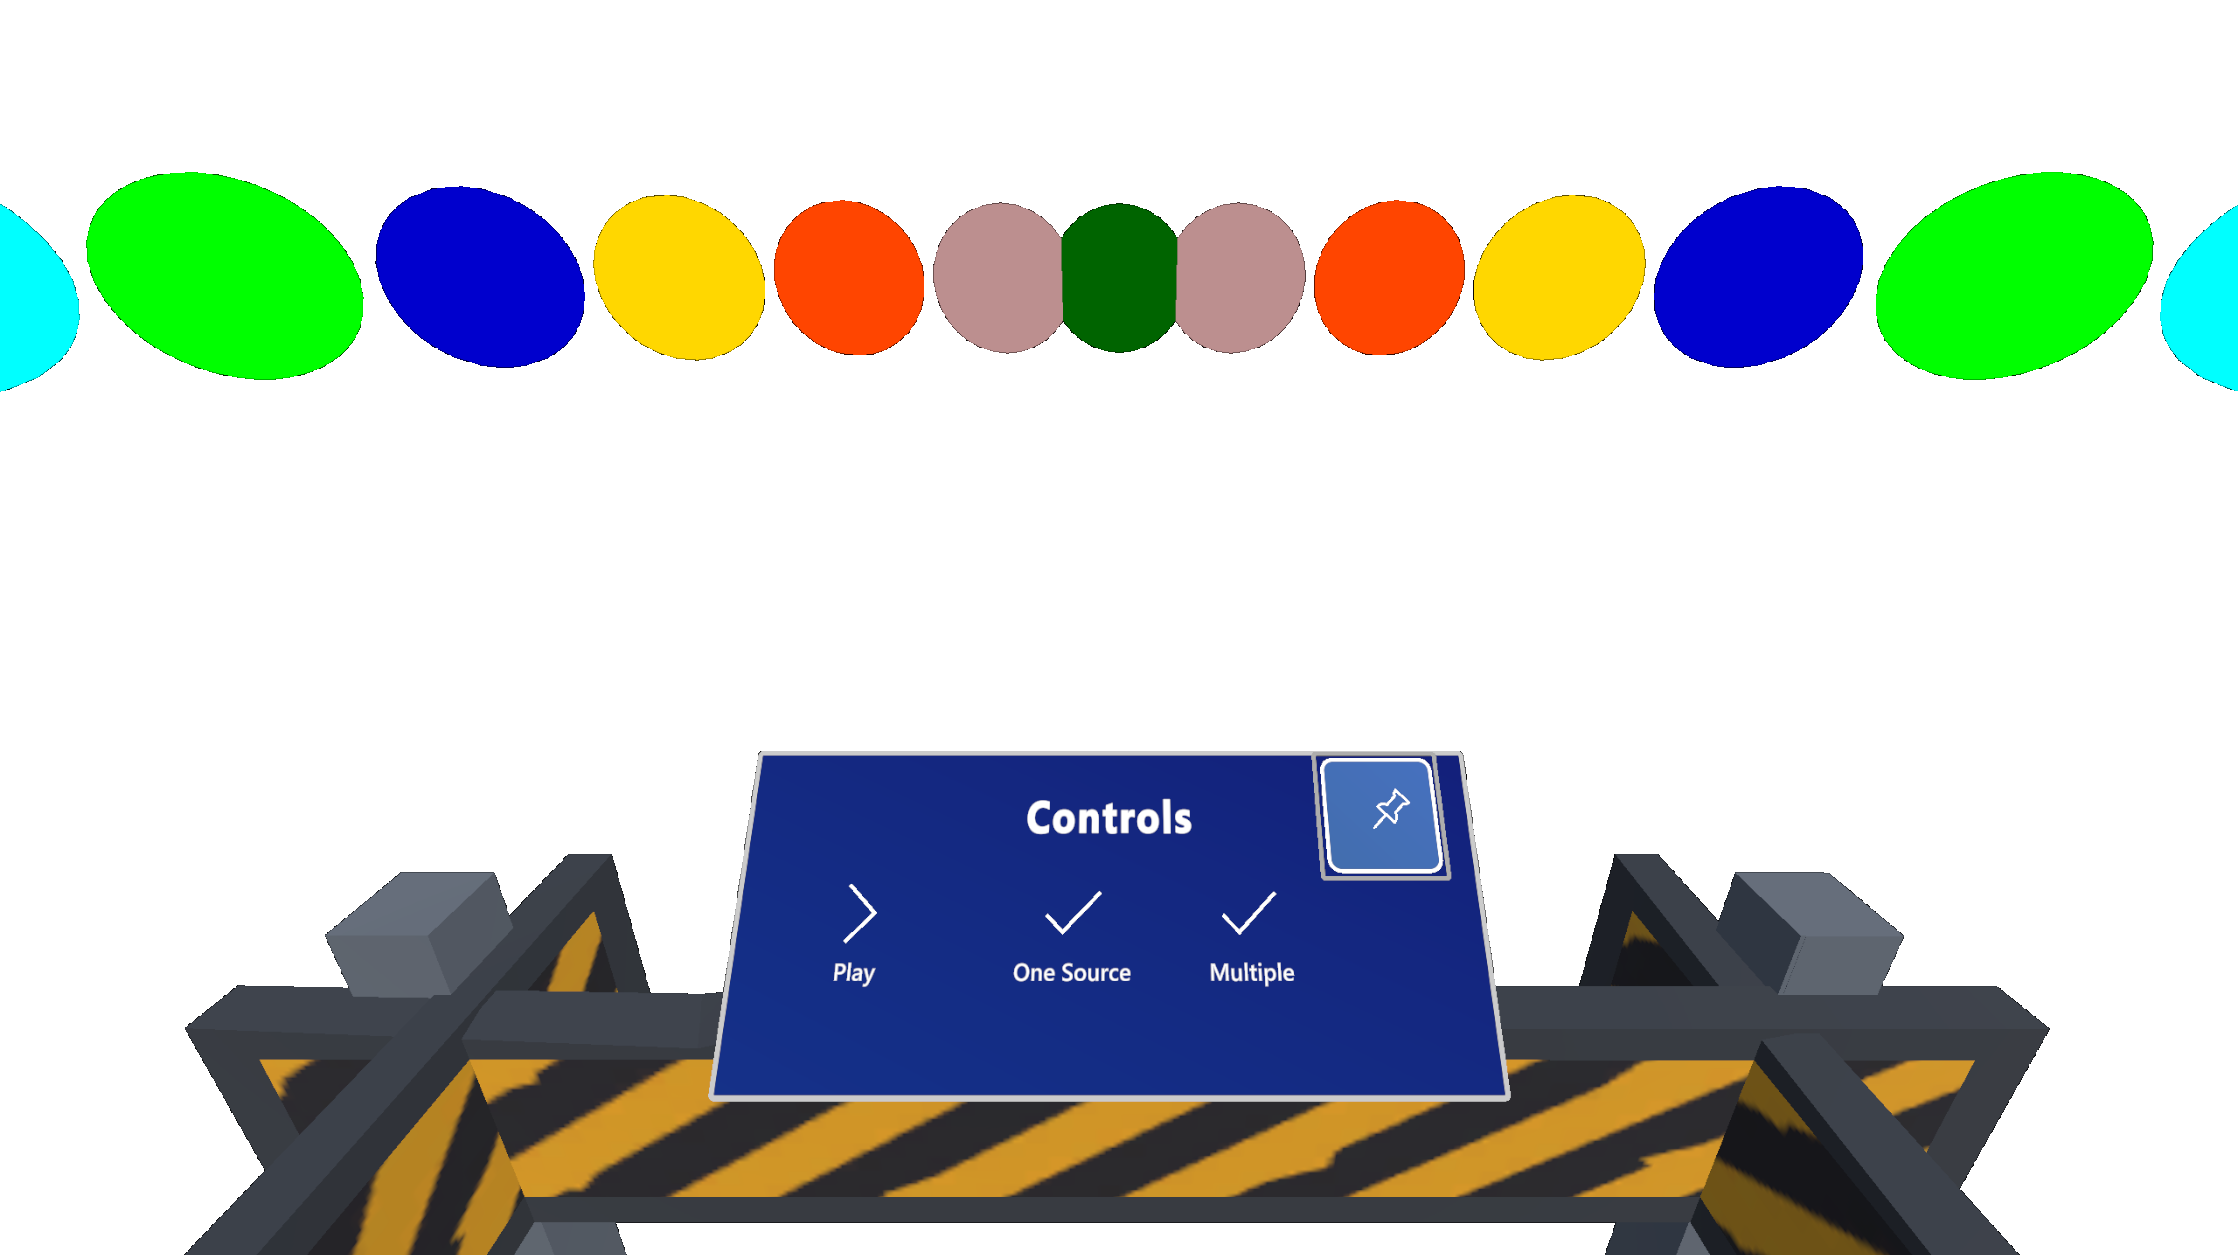
\includegraphics[width=1\columnwidth]{clustering-fpv}
    \caption[Participant's perspective of psychoacoustic testing --- clustering]{First-person view of the clustering task: the participant is presented with spatialised audio that may be emitted by a \emph{single} or \emph{multiple} invisible sound-emitting object(s) and is asked to classify each stimulus using buttons on a holographic panel. The render shows coloured spheres (the perspective camera might affect the appearance of the sphere objects) to visualise the position and distance of sound source pairs; they are invisible to the participants.}\label{fig:clustering-fpv}
\end{figure}
The goal of the \emph{clustering} task is to investigate how well participants can resolve clustered invisible sound sources across the two sets of audio stimuli. The procedure starts with the participant standing on the marker indicated on the floor within the holographic barriers; a holographic panel summarises the task to the participants, and upon interaction with the proceeding button on the panel, the first subtask is administered. For each subtask, the participant is displayed an auditory stimulus and asked to determine whether it is emitted by a \emph{single} or \emph{multiple} invisible sound-emitting object(s). The participant selects one or the other using a panel showing two interactable buttons, ``Single'' and ``Multiple''. \par
Audio stimuli are emitted from a single or pairs of invisible sound sources, represented as colour-coded circles in Figure~\ref{fig:psycho-top-view}. Pairs are positioned along a semicircular array with a radius of $2.24m$, with the listener at the centre of the semicircle. Starting from a singular source in front of the listener at the midpoint of the semicircle, there are eight source pairs with increasing angular distance, about $15$ to $20^\circ$ between pairs. Subtasks are random samplings of the eight sources plus the single source, repeated twice, one for anechoic audio and one for propagated audio. Hence, each participant completes 18 selections.\par

\subsection{Evaluation}
Data collected from procedures is analysed with the goal of evaluating the efficacy of the proposed pipeline and assessing its impact on immersive applications. One of the primary techniques used to compare populations and evaluate significant differences between anechoic stimuli and stimuli generated by the sound rendering pipeline is the Analysis of Variance (ANOVA) or Mann-Whitney U non-parametric test, both particularly useful for comparing the means of multiple groups to determine if there are statistically significant differences among them. In cases where the data do not meet the assumptions required for ANOVA, such as normality or homogeneity of variances, non-parametric tests like the Kruskal-Wallis test are utilised. These tests provide a robust alternative by comparing the medians of the groups, offering insights into whether the sound rendering pipeline produces significantly different auditory experiences compared to anechoic conditions.\par
Another aspect of the evaluation involves measuring localisation error, which assesses the accuracy with which participants can identify the spatial origin of sound sources. This metric is quantified by calculating the angular deviation between the actual and perceived locations of the sound sources. In addition to localisation error, clustering error and accuracy are measured to evaluate how well the participants can group similar sounds together based on their perceived spatial and spectral characteristics. Clustering error is assessed by analysing the consistency of participants' responses in grouping sounds that originate from the same or similar locations. Accuracy is determined by comparing these groupings to the actual configurations of the sound sources. Statistical methods such as cluster analysis and multidimensional scaling are employed to visualize the data and identify patterns. Furthermore, measures like the receiver operating characteristic curve (ROC) can be used to quantify the accuracy between the participant-derived clusters and the true clusters.

\section{Results}
The evaluation framework is deployed to the HMD, and responses are gathered from play sessions with the recruited participants, investigating whether the geometrical acoustics-based rendering pipeline has a significant effect on psychoacoustic-related abilities performed in AR. The overall null hypothesis set for this evaluation is that task performance is not affected by applying approximated acoustic phenomena to auditory stimuli. A total of 3348 responses were drawn from the \emph{localisation} task and 522 responses from the \emph{clustering} task, as two participants withdrew from the latter task. \par

\subsection{Localisation Task}\label{sec:localisation-results}
The observed metric for the \emph{localisation} task is the angular distance between the position of the sound source the participant determines as responsible for reproducing the stimulus and the position of the true sound source, referred to as localisation ``Error'', see Figure~\ref{fig:localisation-distributions}. To determine whether this task is affected by acoustic phenomena applied to auditory stimuli, we set a null hypothesis $H_0$ to determine no significant difference between localisation error samples associated with anechoic audio and localisation error samples associated with propagated audio. \par
The two Error populations are tested for normality to evaluate whether the assumptions for conducting variance tests by setting a hypothesis $H_n$ determine that the two populations come from a normal distribution \citep{pearson1977tests}. Normality tests fail to prove $H_n$ for both distributions with $7.9\ *\ 10^2$, $7.3\ *\ 10^2$ statistical scores and $\rho\ =\ 6.2\ *\ 10^{-17}$, $\rho\ =\ 3.4\ *\ 10^{-158}$ significance values for Error samples associated with the \emph{anechoic} and \emph{pipeline} stimulus sets, respectively. Given the departure from normality in the recorded responses, the Mann-Whitney U non-parametric test is used to compare the distributions, rejecting $H_0$ with $1.34\ *\ 10^6\ U$ score and $\rho\ =\ 0.042$ significance value. The significance value threshold is set at $0.05$ for all hypotheses. \par

\begin{table}[htbp]
\centering
\caption{The table shows mean, mean standard error, standard deviation, variance score, kurtosis, and skewness factors computed on \textbf{distances} between true values and responses indicated by subjects performing the localisation task across the two sets of audio stimuli, anechoic $S_A$ and pipeline-generated $S_P$. These distances measure the angle between the position of the object responsible for propagating sounds and the object the participants deemed responsible for propagating sounds. The Standard Error for Kurtosis and Skewness scores are, respectively, 0.2 and 0.1 across all distances for both $S_A$ and $S_P$.}\label{tab:loc-error-groups}
\begin{tabular}{@{}llllllll@{}}
\toprule
Distance                & Stimulus Set & $\mu$   & S.E.$\mu$ & $\sigma$ & Variance & Kurtosis & Skewness    \\ \midrule
\multirow{2}{*}{Near}   & $S_A$ & 30.93          & 1.62      & 38.03   & 1446.32  & 4.6        & 2.32       \\
                        & $S_P$ & \textbf{24.76} & 1.37      & 31.55   & 995.56   & 7.24       & 2.76       \\
\multirow{2}{*}{Medium} & $S_A$ & 24.85          & 1.77      & 42.11   & 1773.43  & 4.08       & 2.17       \\
                        & $S_P$ & \textbf{21.36} & 1.53      & 37.22   & 1385.09  & 5.58       & 2.4        \\
\multirow{2}{*}{Far}    & $S_A$ & \textbf{22.84} & 1.89      & 44.67   & 1995.84  & 4.38       & 2.28       \\
                        & $S_P$ & 25.16          & 1.92      & 45.28   & 2050.01  & 3.32       & 2.04       \\ \bottomrule
\end{tabular}
\end{table}

\begin{figure}[htbp]
    \centering
    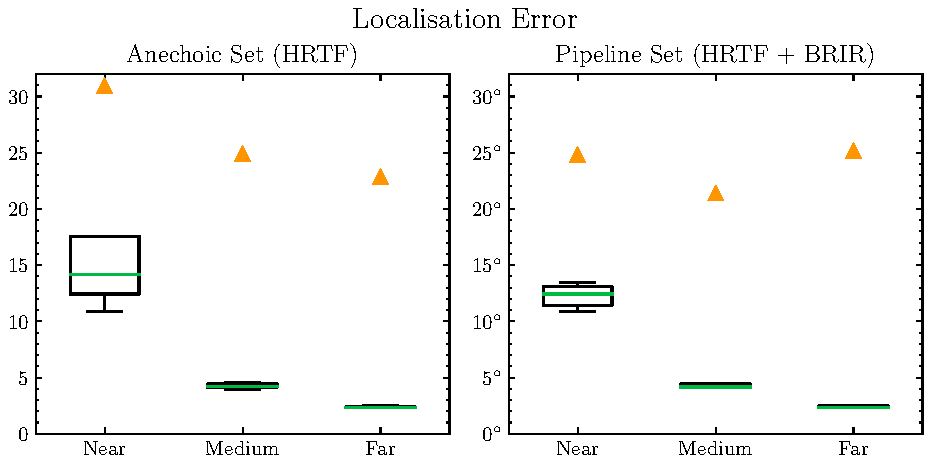
\includegraphics[width=1\linewidth]{localisation_accuracy}
    \caption[Psychoacoustic test results --- localisation error]{Boxplots comparing localisation errors across near, medium, and far sound source distances, showing Interquartile range (the box), the median value (the green line), and the mean value for each group, across the $S_A$ and $S_P$ stimulus sets.}\label{fig:localisation-acc}
\end{figure}

\begin{figure}[htbp]
    \centering
    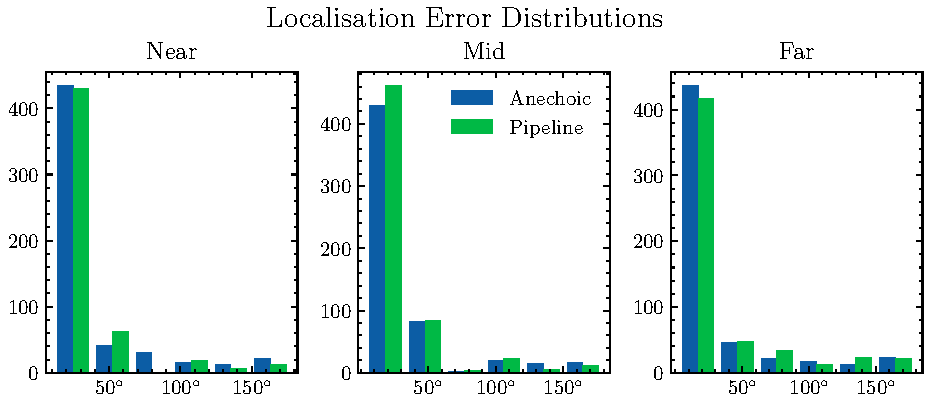
\includegraphics[width=1\linewidth]{localisation_distributions}
    \caption[Psychoacoustic test results --- localisation accuracy distributions]{Distributions of angular errors sampled from the localisation task, shown across the distance between listener and array of sound sources. The histograms compare samples from the set of anechoic audio stimuli and samples from the set of stimuli generated with the deployed geometrical acoustics-based rendering pipeline. Both sample sets have stimuli conveyed to participants using individualised HRTFs and maintain the same spatialisation apparatus.}\label{fig:localisation-distributions}
\end{figure}

\subsection{Clustering Task}
The observed metric for the \emph{clustering} task is the rate of correct answers provided by subjects for each subtask, where they are asked to identify whether a single or multiple invisible sources emit the sound. The responses are analysed as a binary classification task, measuring accuracy and precision across the two stimulus sets. Table~\ref{tab:f1-masking} shows the accuracy of sound source cluster classification for two stimulus sets and their union across all angular distances between sources in each pair.
\begin{figure}[htbp]
    \centering
    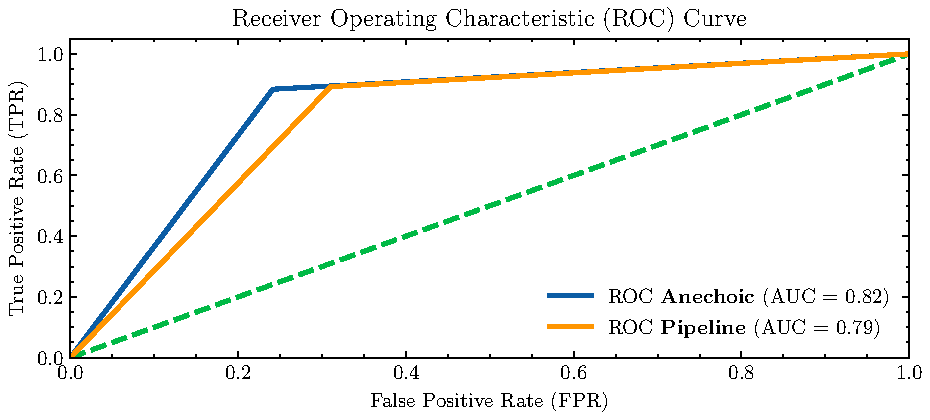
\includegraphics[width=1\linewidth]{masking_roc}
    \caption[Psychoacoustic test results --- clustering accuracy]{Receiver Operating Characteristic (ROC) curves showing the success rate and false positive of responses provided by participants indicating whether perceived audio stimuli are emitted by a singular or multiple invisible sound-emitting objects placed in the testing scene.}\label{fig:masking-roc}
\end{figure}

\begin{table}[htbp]
\centering
\begin{tabular}{@{}llll@{}}
\toprule
Angle       & $F_1$ Anechoic & $F_1$ Pipeline & $F_1$ Aggregate \\ \midrule
$143^\circ$ & 1.0            & 1.0            & 1.0             \\
$125^\circ$ & 1.0            & 1.0            & 1.0             \\
$106^\circ$ & 1.0            & 1.0            & 1.0             \\
$ 88^\circ$ & 0.97           & 1.0            & 0.98            \\
$ 69^\circ$ & 1.0            & 1.0            & 1.0             \\
$ 51^\circ$ & 1.0            & 0.72           & 0.86            \\
$ 33^\circ$ & 0.59           & 0.9            & 0.74            \\
$ 14^\circ$ & 0.52           & 0.52           & 0.52            \\
$  0^\circ$ & 0.76           & 0.69           & 0.72            \\ \bottomrule
\end{tabular}
\caption[Psychoacoustic test results --- clustering scores]{$F_1$ score evaluated over responses gathered from the clustering test, expressing participants' accuracy in discriminating single and multiple invisible sound-emitting objects at increasing angular distances. Scores are computed over the set of anechoic audio stimuli $S_A$; audio stimuli generated from the pipeline $S_P$ and their aggregate.}\label{tab:f1-masking}
\end{table}

\section{Discussion}
The overarching goal of this research is to investigate whether approximated acoustic phenomena applied to auditory interactions in AR affect task performance for activities related to psychoacoustic abilities performed naturally by the Human Hearing System.
The comparison of distributions with a non-parametric test shows a significant difference between responses associated with the anechoic set $S_A$ and the pipeline set $S_P$, as presented in Section~\ref{sec:localisation-results}. The approximated acoustic reverberation convolved to unpropagated audio computed by a ray tracer is sufficient to affect the perception of spatial resolution of sound-emitting objects in AR. However, comparing means of angular error distributions across distances from the listener shows that as the distance from the sound source increases, this effect hinders the spatial resolution abilities of subjects. \par
The localisation accuracy drops as the distance increases, as shown in Table~\ref{tab:loc-error-groups}, with the angular error favouring the anechoic stimulus set for far sound sources. The significance of the results gathered from the localisation task aligns with \cite{rungta2016psychoacoustic}'s work, demonstrating that physically accurate acoustic simulations have a perceptual impact on tasks in virtual environments. For the space in question, approximations of acoustic phenomena, computed with only $3*10^3$ rays and fourth-order reflections, affect task performance in AR for activities related to psychoacoustic abilities, hence determining that stimulus sets produced using the acoustic rendering pipeline affect matching of visual-acoustic information. \par
The analysis conducted on responses gathered from the clustering task indicates that acoustic responses allow subjects to better resolve clustered sound sources. Figure~\ref{fig:masking-roc} shows better classification performance in subjects utilising the \emph{pipeline} stimulus set. However, this is only true for clustered sources that are farther than $15^\circ$ apart.
The practical implications of this study lie within the ability to design future auditory interactions in AR. When designing tasks in AR involving the application of psychoacoustic abilities, such as pinpointing the position of sound-emitting objects or resolving the nature of concurrent sound sources, acoustic modelling based on a virtual reconstruction of the space can suffice to affect task performance. From this practical implication stems the main theoretical contribution that transfers the established psychoacoustic characterisation of sound propagation effects to AR space, which has unlocked new potential in the realm of audio interactions. However, the theoretical contribution will require a set of complex scenes with diverse architectural and acoustic characteristics, evaluating the generalisability of the findings discussed in this work. \par
Despite the limited generalisability, there are important new research directions that branch from these results: mainly the need for an end-to-end pipeline for acoustic rendering in AR based on spatial understanding technology supplied by HMDs and the relationship between auditory interactions in AR and acoustic phenomena modelled from spatial understanding. The latter could have a potential impact on improving task performance in reverberant spaces since the data gathered shows that distance and reverberant sources can impact localisation, future research would explore whether physical sound sources can be affected by cross-talk cancellation techniques to remove wet components from signals, addressing such impact wherever negative. Such techniques could be based on real-time modelling techniques, such as neural networks for IR generation or acoustic novel view synthesis recently pioneered by \cite{ratnarajah2022mesh2ir} and  \cite{chen2023novel}, to improve clarity and definition of auditory interactions with inverse rendering approaches. \par

\subsection{Significance}
The results demonstrate that the proposed audio rendering pipeline enhances localisation resolution and allows better resolution of masking effects in audio stimuli within \acrshort{ar} environments. Due to the ability of audio stimuli of conveying scene information, this can have an effect on the wider domains that leverage spatial audio in immersive environments \citep{yang2022audio}. 
The ability to accurately localise sound sources within an \acrshort{ar} environment is crucial for many applications. Improved spatial awareness can enhance user interactions in training simulations for medical and military applications, where precise sound localisation can be critical for success \citep{vine2023training}. For instance, in medical training, the ability to pinpoint the origin of alarms or equipment sounds can improve response times and decision-making. Enhanced audio realism contributes to a more immersive and natural user experience. In the entertainment and gaming industries, where user engagement is paramount, realistic audio cues that correspond accurately to visual elements can significantly boost the overall experience \citep{slater2009visual}.


\section{Conclusions}
This research has explored the psycho-acoustic characterisation of geometrical acoustics-based rendering pipelines in AR, providing a novel lens through which the auditory interactions in AR environments can be understood and enhanced. The designed study revealed the criticality of integrating fundamental acoustic principles to augment the realism and immersive quality of auditory experiences in AR environments --- illuminating the necessity in the proposed pipeline to deliver more correct human responses to acoustic tasks within AR contexts. \par
The research involved human participants to enable us to decipher the efficacy of sound rendering techniques in AR, particularly focusing on their capacity to emulate psycho-acoustic abilities. Through the experimental design, the study illuminated the nuances of sound transmission in AR contexts, providing a large dataset enabling comparative analysis of performance in psycho-acoustic tasks, localisation and clustering. \par
The contributions of this work were threefold: firstly, it introduced a pioneering methodology for studying psycho-acoustic factors within simulated sound fields in AR; secondly, it developed a bespoke testing framework, employing a custom audio engine and a prototype acoustic rendering pipeline for an AR context, facilitating AR evaluation; and thirdly, it provided insightful recommendations for the future design of audio rendering pipelines in immersive technology, derived from a comprehensive data-set of perceptual responses. \par
The findings underscored the significant impact of acoustic approximations and spatial understanding in enhancing auditory interactions in AR, revealing that the convolution of approximated acoustic phenomena to audio stimuli can notably influence psycho-acoustic abilities and potentially modulate task performance in AR applications. This research not only paves the way for further exploration into sound rendering in AR but also establishes a foundational framework for developing more immersive and acoustically precise or beneficial AR applications across various domains. \par
The experimental evaluation explores the first steps towards the question concerning subjective factors affected by the deployment of a context-aware acoustic rendering pipeline, showing significant differences in stimuli considering approximated acoustic phenomena against unpropagated audio. Future work may seek to explore the application and impact of these findings across diverse AR platforms and user demographics, thereby enriching our understanding and development of acoustically immersive and perceptually coherent AR environments. Important next steps towards defining the relationship between vision-based acoustic pipelines and auditory interactions in AR should aim at defining the requirements from both the acoustic rendering and the acoustic characteristic retrieval, performing ablation studies on both components to evaluate Just-Noticeable differences across acoustic rendering resolution levels or to evaluate the required granularity of acoustic characteristics to be attributed to the scene geometry.
